\documentclass[12pt,a4paper,titlepage]{article}
\usepackage[utf8]{inputenc}
\usepackage[finnish]{babel}
\usepackage{setspace}
\usepackage{parskip}
\usepackage{amssymb}
\usepackage{amsmath}
\usepackage{graphicx}
\usepackage{fancyhdr}
\usepackage[top=1in, bottom=1in, left=1in, right=1in]{geometry}
\usepackage{float}
\usepackage[section]{placeins}
%\usepackage[numbered,autolinebreaks,useliterate]{mcode} % jos tahdot laittaa matlabkoodia näkyville niin kannattaa käyttää tätä

% hyödyllisiä paketteja:
\usepackage{siunitx}\sisetup{per=frac} % SI-yksiköitä.
%\usepackage{supertabular} % jos tarttee isoja taulukoita
%\usepackage{fullpage} % pienemmät marginaalit jos haluaa

\usepackage{hyperref} % lisääthän omat pakettisi ENNEN hyperref'iä
\hypersetup{pdfborder={0 0 0}}
\onehalfspacing
\cfoot{}
\rhead{\thepage}
% asettaa nyk. kappaleen nimen vasempaan ylänurkkaan, saa poistaa jos haluaa
\lhead{\leftmark}

\usepackage{bm}
\newcommand{\matr}[1]{\bm{#1}}
\newcommand{\transpose}[1]{{#1}^T}

%%%%% kaikki ennen tätä liittyy käytettäviin paketteihin tai dokumentin muotoiluun. siihen ei tarvinne aluksi koskea. %%%%%

%%%%% kansilehti %%%%%
\title{Taivaanmekaniikka \\ Lineaarinen pienimmän neliösumman sovitus \vspace{0.5em}}
\author{\begin{tabular}{c}
Anni Järvenpää
\end{tabular}}
\date{\today}
\begin{document}
\maketitle

%%%%%%%%%%%%%%% Oleellinen sisältö alkaa%%%%%%%%%%%%%%%
\section{Lineaarinen pienimmän neliösumman menetelmä}
Lineaarisen pienimmän neliösumman menetelmän tavoitteena on sovittaa $n$ muotoa $(x_i, y_i)$ olevasta pisteestä koostuvaan havaintoaineistoon suora, joka edustaa pisteitä mahdollisimman hyvin. Tyypillisesti sovituksen hyvyyttä mitataan pisteiden vertikaalisena etäi\-syytenä~$|e|$ sovitetusta suorasta (merkitty sinisellä kuvassa \ref{vertikaalietaisyys}). Pienimmän neliösumman menetelmässä näiden vertikaalisten poikkeamien neliöiden summa pyritään minimoimaan, siis etsimään funktion $f(x) = \beta_1 + \beta_2 x + \beta_3 x^2 + ... + \beta_{m+1} x^m$ kertoimet $\beta_1 ... \beta_{m+1}$ siten, että virhe $S$ on mahdollisimman pieni, kun $S$ on määritelty yhtälön \ref{virhe} mukaisesti.~\cite{basicideas}
\begin{equation} \label{virhe}
	S = \sum\limits_{i=1}^{n} e_i^2 = \sum\limits_{i=1}^{n} (y_i - f(x_i))^2
\end{equation}

\begin{figure}
\centering
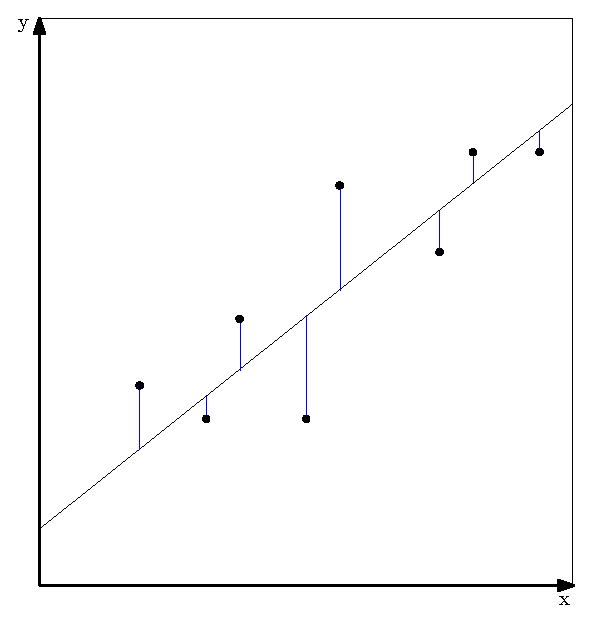
\includegraphics{vertikaalietaisyys.eps}
\caption{Pistejoukko, johon sovitettu suora mustalla ja pisteiden vertikaaliset etäisyydet suorasta pisteinä.}
\label{vertikaalietaisyys}
\end{figure}

Virheen minimiarvot löytyvät derivaatan nollakohdista:
\begin{align*}
	\frac{\partial R^2}{\partial \beta_1} &= -2\sum\limits_{i=1}^n[y-(\beta_1+\beta_2x+...+\beta_{m+1}x^m)]=0 \\
	\frac{\partial R^2}{\partial \beta_2} &= -2\sum\limits_{i=1}^n[y-(\beta_1+\beta_2x+...+\beta_{m+1}x^m)]=0 \\
	&\vdots  \\
	\frac{\partial R^2}{\partial \beta_{m+1}} &= -2\sum\limits_{i=1}^n[y-(\beta_1+\beta_2x+...+\beta_{m+1}x^m)]=0
\end{align*}
Näistä saadaan edelleen 
\begin{align*}
	\beta_1 n+\beta_2\sum\limits_{i=1}^n x_i+...+\beta_{m+1} \sum\limits_{i=1}^n x_i^m &= \sum\limits_{i=1}^n y_i \\
	\beta_1\sum\limits_{i=1}^nx_i+\beta_1\sum\limits_{i=1}^nx_i^2+...+\beta_{m+1}\sum\limits_{i=1}^nx_i^{m+1} &= \sum\limits_{i=1}^n x_iy_i  \\
	\beta_1\sum\limits_{i=1}^nx_i^{m}+\beta_1\sum\limits_{i=1}^nx_i^{m+1}+...+\beta_{m+1}\sum\limits_{i=1}^nx_i^{2m} &= \sum\limits_{i=1}^n x_i^{m}y_i
\end{align*}
eli matriisimuodossa
\begin{equation*}
	\begin{bmatrix}
		n & \sum\limits_{n=1}^{n} x_i & ... & \sum\limits_{n=1}^{n} x_i^{m} \\
		\sum\limits_{n=1}^{n} x_i & \sum\limits_{n=1}^{n} x_i^2 & ... & \sum\limits_{n=1}^{n} x_i^{m+1} \\
		\vdots & \vdots & \ddots  & \vdots \\
		\sum\limits_{n=1}^{n} x_i^{m} & \sum\limits_{n=1}^{n} x_i^{m+1} & ... & \sum\limits_{n=1}^{n} x_i^{2m}
	\end{bmatrix}
	\begin{bmatrix}
		\beta_1 \\
		\beta_2 \\
		\vdots \\
		\beta_{m} \\
		\beta_{m+1} \\
	\end{bmatrix}
	=
	\begin{bmatrix}
		\sum\limits_{i=1}^n y_1 \\
		\sum\limits_{i=1}^n y_2 \\
		\vdots \\
		\sum\limits_{i=1}^n y_{m} \\
	\end{bmatrix}
\end{equation*}
Tämä voidaan edelleen kirjoittaa~\cite{wolframmath}
\begin{equation} \label{matriiseilla}
	\begin{bmatrix}
		x_{1}^0 & x_{1}^2 & ...    & x_{1}^n \\
		x_{2}^0 & x_{2}^2 & ...    & x_{2}^n \\
		\vdots  & \vdots  & \ddots & \vdots  \\
		x_{m}^0 & x_{m}^2 &    ... & x_{m}^n
	\end{bmatrix}
	\begin{bmatrix}
		\beta_1 \\
		\beta_2 \\
		\vdots \\
		\beta_{m+1} \\
	\end{bmatrix}
	=
	\begin{bmatrix}
		y_1 \\
		y_2 \\
		\vdots \\
		y_n
	\end{bmatrix}
\end{equation}

Merkitään nyt
\begin{equation*}
	\matr{Y} =
		\begin{bmatrix}
			y_1 \\
			y_2 \\
			\vdots \\
			y_n
		\end{bmatrix},\qquad
	\matr{X} = 
		\begin{bmatrix}
			x_{1}^0 & x_{1}^2 & ...    & x_{1}^n \\
			x_{2}^0 & x_{2}^2 & ...    & x_{2}^n \\
			\vdots  & \vdots  & \ddots & \vdots  \\
			x_{m}^0 & x_{m}^2 &    ... & x_{m}^n
		\end{bmatrix} \quad \text{ja} \quad
	\matr{\beta} =
		\begin{bmatrix}
			\beta_1 \\
			\beta_2 \\
			\vdots \\
			\beta_m			
		\end{bmatrix},
\end{equation*}
jolloin yhtälö \ref{matriiseilla} saadaan seuraavaan muotoon, josta voidaan helposti ratkaista $\matr{\beta}$.~\cite{wolframmath}
\begin{alignat}{2}
	\matr{Y} &= \matr{X}\matr{\beta} &&|| \transpose{\matr{X}} \cdot \nonumber \\
	\transpose{\matr{X}}\matr{Y} &= \transpose{\matr{X}}\matr{X}\matr{\beta} &&|| (\transpose{\matr{X}}\matr{X}\matr{\beta})^{-1} \nonumber \\
	\matr{\beta} &= (\transpose{\matr{X}}\matr{X})^{-1}\matr{X}\matr{Y} \quad &&
\end{alignat}


%%%%% Sisältö loppuu, lähdeluettelo %%%%%
\newpage
\bibliographystyle{plain}
\bibliography{lahteet} 
\appendix
\newpage
\section{Liittyvä liite.} \label{koodi}
Liian laaja leipätekstiin.
\end{document}
